\chapter{Resultados de las Otras Series Reales}
\label{aneD_00_00_otras_series}

% Corridas 103-107 de notebooks/reales/, M = 10, test, w = 30. Cuadros desde reports/reales/<eid>_barrido_M/{98,99,102}_*
% y <eid>_m10/{72,81}_ventana_*_w30.csv (scratchpad tablas_aneD.py); figuras con el estilo del Capítulo 3 (figuras_aneD.py).

Este anexo reúne los resultados del PSBPM-FD en otras cinco series reales de curvas diarias, ajustadas con la misma configuración que el tráfico con el rezago de un día (Capítulo~\ref{04_00_00_aplicacion}). A diferencia del tráfico, ninguna de ellas tiene un estado oculto que separe perfiles distintos de la curva siguiente, y en todas la predictiva resultó unimodal. Se reportan el error puntual, los intervalos de predicción y, brevemente, los comportamientos predictivos. Salvo indicación, las cifras corresponden a $M = 10$, al bloque de prueba y a la ventana móvil de ancho $w = 30$.

\section{Series y configuración}
\label{aneD_00_01_series}

El Cuadro~\ref{tab:aneD_series} describe las series. Cada día es una curva observada en $G$ instantes, a la que se aplica, cuando se indica, una transformación que estabiliza su escala, y las métricas se calculan en la escala transformada. La configuración es la del tráfico con el rezago de un día (Cuadro~\ref{tab:aneC_configuracion}): base B-spline cúbica de $K = 10$ funciones con el mismo tratamiento de los huecos, FPCA estimada con el bloque de entrenamiento, $M = 10$ componentes, los diez scores del día anterior como covariables de cada score, $a_\nu = 2$, inclusión a priori $(1, 5)$ y una cadena de 2500 iteraciones con 30 átomos. La única diferencia es el calentamiento, de 500 iteraciones en lugar de 1000. Las referencias son el FAR(1), con su banda gaussiana, y el Random Forest con las mismas covariables.

% Fuente: datasets_manifest.json y 65_comportamientos_calendario.csv de cada corrida; descripción de la curva en el _01.
\begin{table}[H]
\centering\small
\setlength{\tabcolsep}{3.5pt}
\caption{Series reales adicionales: variable de la curva diaria, número de instantes por día ($G$), período, número de días ($T$) y partición en entrenamiento y prueba.}
\label{tab:aneD_series}
\begin{tabular}{l p{0.36\textwidth} c c c c}
\hline
Serie & Curva diaria & $G$ & Período & $T$ & Entren. / prueba \\
\hline
Precio SA1 & Precio spot de la región Australia del Sur del mercado eléctrico australiano (AEMO), $\operatorname{asinh}(\text{precio}/100)$, cada 5 minutos & 288 & 2022--2025 & 1461 & 1096 / 365 \\
PM2.5 O'Higgins & Concentración horaria de PM2.5 en la estación Parque O'Higgins de Santiago (SINCA), $\log(1 + x)$ & 24 & 2015--2025 & 4018 & 2922 / 1096 \\
PM2.5 Beijing & Concentración horaria de PM2.5, promedio de doce estaciones de Beijing, $\log(1 + x)$ & 24 & 2013--2017 & 1461 & 1022 / 439 \\
Eólica & Factor de planta de la generación eólica terrestre de Alemania (SMARD), cada 15 minutos & 96 & 2015--2026 & 4299 & 3009 / 1290 \\
Volatilidad BTC & Mitad del logaritmo de la varianza realizada horaria de BTCUSDT (Binance), con retornos de 5 minutos & 24 & 2020--2026 & 2435 & 1704 / 731 \\
\hline
\end{tabular}
\end{table}

\section{Error puntual}
\label{aneD_00_02_error_puntual}

Los Cuadros~\ref{tab:aneD_bloqueA} a~\ref{tab:aneD_bloqueA_gana} resumen el MAE y el RMSE de los tres predictores del PSBPM-FD y de las dos referencias, como en la Sección~\ref{04_03_01_error_puntual}. Como las escalas de las series son distintas, las cifras se comparan dentro de cada fila y no entre series.

% Fuente: 98_resumen_bloqueA_min_max_prom.csv del barrido (test, M = 10, promedio sobre ventanas).
\begin{table}[H]
\centering\small
\setlength{\tabcolsep}{3pt}
\caption{MAE y RMSE en el bloque de prueba por serie ($M = 10$, $w = 30$). En negrita el menor de cada métrica.}
\label{tab:aneD_bloqueA}
\begin{tabular}{l ccccc ccccc}
\hline
 & \multicolumn{5}{c}{MAE} & \multicolumn{5}{c}{RMSE} \\
Serie & Esp. & Med. & Modal & RF & FAR & Esp. & Med. & Modal & RF & FAR \\
\hline
Precio SA1 & \textbf{0.3279} & 0.3286 & 0.3438 & 0.3415 & 0.3280 & \textbf{0.4417} & 0.4430 & 0.4666 & 0.4528 & 0.4418 \\
PM2.5 O'Higgins & \textbf{0.3166} & 0.3168 & 0.3327 & 0.3281 & 0.3214 & \textbf{0.4300} & 0.4311 & 0.4526 & 0.4459 & 0.4347 \\
PM2.5 Beijing & 0.5664 & 0.5515 & 0.5786 & 0.5957 & \textbf{0.5506} & 0.7445 & 0.7503 & 0.8385 & 0.7606 & \textbf{0.7390} \\
Eólica & 0.0859 & \textbf{0.0853} & 0.0993 & 0.0961 & 0.0857 & \textbf{0.1191} & 0.1196 & 0.1368 & 0.1270 & 0.1197 \\
Volatilidad BTC & 0.3288 & 0.3303 & 0.3489 & 0.3292 & \textbf{0.3242} & 0.4229 & 0.4247 & 0.4466 & 0.4230 & \textbf{0.4184} \\
\hline
\end{tabular}
\end{table}

\begin{table}[H]
\centering\small
\setlength{\tabcolsep}{3.5pt}
\caption{Cambio relativo del MAE y del RMSE respecto del FAR por predictor y serie. Negativo es mejor que el FAR.}
\label{tab:aneD_bloqueA_ganancia}
\begin{tabular}{l cc cc cc cc}
\hline
 & \multicolumn{2}{c}{Esperanza} & \multicolumn{2}{c}{Mediana puntual} & \multicolumn{2}{c}{Átomo más probable} & \multicolumn{2}{c}{Random Forest} \\
Serie & MAE & RMSE & MAE & RMSE & MAE & RMSE & MAE & RMSE \\
\hline
Precio SA1 & $0.0\%$ & $0.0\%$ & $+0.2\%$ & $+0.3\%$ & $+4.8\%$ & $+5.6\%$ & $+4.1\%$ & $+2.5\%$ \\
PM2.5 O'Higgins & $-1.5\%$ & $-1.1\%$ & $-1.4\%$ & $-0.8\%$ & $+3.5\%$ & $+4.1\%$ & $+2.1\%$ & $+2.6\%$ \\
PM2.5 Beijing & $+2.9\%$ & $+0.7\%$ & $+0.2\%$ & $+1.5\%$ & $+5.1\%$ & $+13.5\%$ & $+8.2\%$ & $+2.9\%$ \\
Eólica & $+0.3\%$ & $-0.5\%$ & $-0.4\%$ & $-0.1\%$ & $+15.9\%$ & $+14.3\%$ & $+12.1\%$ & $+6.1\%$ \\
Volatilidad BTC & $+1.4\%$ & $+1.1\%$ & $+1.9\%$ & $+1.5\%$ & $+7.6\%$ & $+6.7\%$ & $+1.5\%$ & $+1.1\%$ \\
\hline
\end{tabular}
\end{table}

% Fuente: 72_ventana_modelos_w30.csv (test, sin ventanas que cruzan T0, sin el medoide).
\begin{table}[H]
\centering\small
\setlength{\tabcolsep}{3.5pt}
\caption{Fracción de ventanas de prueba que gana cada modelo, por MAE y por RMSE.}
\label{tab:aneD_bloqueA_ventanas}
\begin{tabular}{l ccccc ccccc}
\hline
 & \multicolumn{5}{c}{MAE} & \multicolumn{5}{c}{RMSE} \\
Serie & FAR & RF & Esp. & Med. & Modal & FAR & RF & Esp. & Med. & Modal \\
\hline
Precio SA1 & 45\% & 16\% & 23\% & 11\% & 4\% & 48\% & 25\% & 22\% & 4\% & 1\% \\
PM2.5 O'Higgins & 22\% & 17\% & 31\% & 26\% & 4\% & 25\% & 19\% & 28\% & 26\% & 1\% \\
PM2.5 Beijing & 40\% & 9\% & 5\% & 29\% & 19\% & 45\% & 14\% & 23\% & 17\% & 0\% \\
Eólica & 39\% & 4\% & 12\% & 40\% & 6\% & 34\% & 9\% & 23\% & 29\% & 5\% \\
Volatilidad BTC & 52\% & 28\% & 17\% & 2\% & 1\% & 50\% & 32\% & 14\% & 3\% & 0\% \\
\hline
\end{tabular}
\end{table}

\begin{table}[H]
\centering\small
\setlength{\tabcolsep}{3.5pt}
\caption{Fracción de ventanas de prueba en que el predictor consistente del PSBPM-FD supera a cada referencia: la mediana puntual bajo MAE y la esperanza bajo RMSE.}
\label{tab:aneD_bloqueA_gana}
\begin{tabular}{l cc cc}
\hline
 & \multicolumn{2}{c}{MAE (mediana puntual)} & \multicolumn{2}{c}{RMSE (esperanza)} \\
Serie & vs FAR & vs RF & vs FAR & vs RF \\
\hline
Precio SA1 & 41\% & 82\% & 43\% & 74\% \\
PM2.5 O'Higgins & 69\% & 77\% & 67\% & 79\% \\
PM2.5 Beijing & 54\% & 86\% & 43\% & 74\% \\
Eólica & 55\% & 95\% & 56\% & 90\% \\
Volatilidad BTC & 18\% & 46\% & 23\% & 52\% \\
\hline
\end{tabular}
\end{table}

En el error puntual la esperanza y la mediana puntual del PSBPM-FD quedan a menos de un $3\%$ del FAR en todas las series. La ventaja más clara es la del PM2.5 de Parque O'Higgins, donde la esperanza baja el MAE y el RMSE del FAR en un $1.5\%$ y un $1.1\%$ y el predictor consistente le gana en dos de cada tres ventanas. En el precio SA1 y en la eólica el empate es casi exacto, con diferencias de medio punto porcentual o menos, mientras que en el PM2.5 de Beijing y en la volatilidad de BTC el FAR es el mejor, con la mayor distancia en la volatilidad, donde la mediana puntual le gana solo en el $18\%$ de las ventanas. Como las predictivas son unimodales, la esperanza y la mediana puntual casi coinciden, y solo en Beijing se separan, con una mediana que baja el MAE de la esperanza en un $2.6\%$, señal de una predictiva asimétrica. El átomo más probable es el peor predictor del PSBPM-FD en todas las series, como en el estudio de simulación. El Random Forest queda por detrás del FAR en las cinco series, y el predictor consistente del PSBPM-FD lo supera en la mayoría de las ventanas salvo en la volatilidad de BTC, donde ambos empatan.

% Fuente: 72_ventana_modelos_w30.csv de cada serie (test).
\begin{figure}[H]
\centering
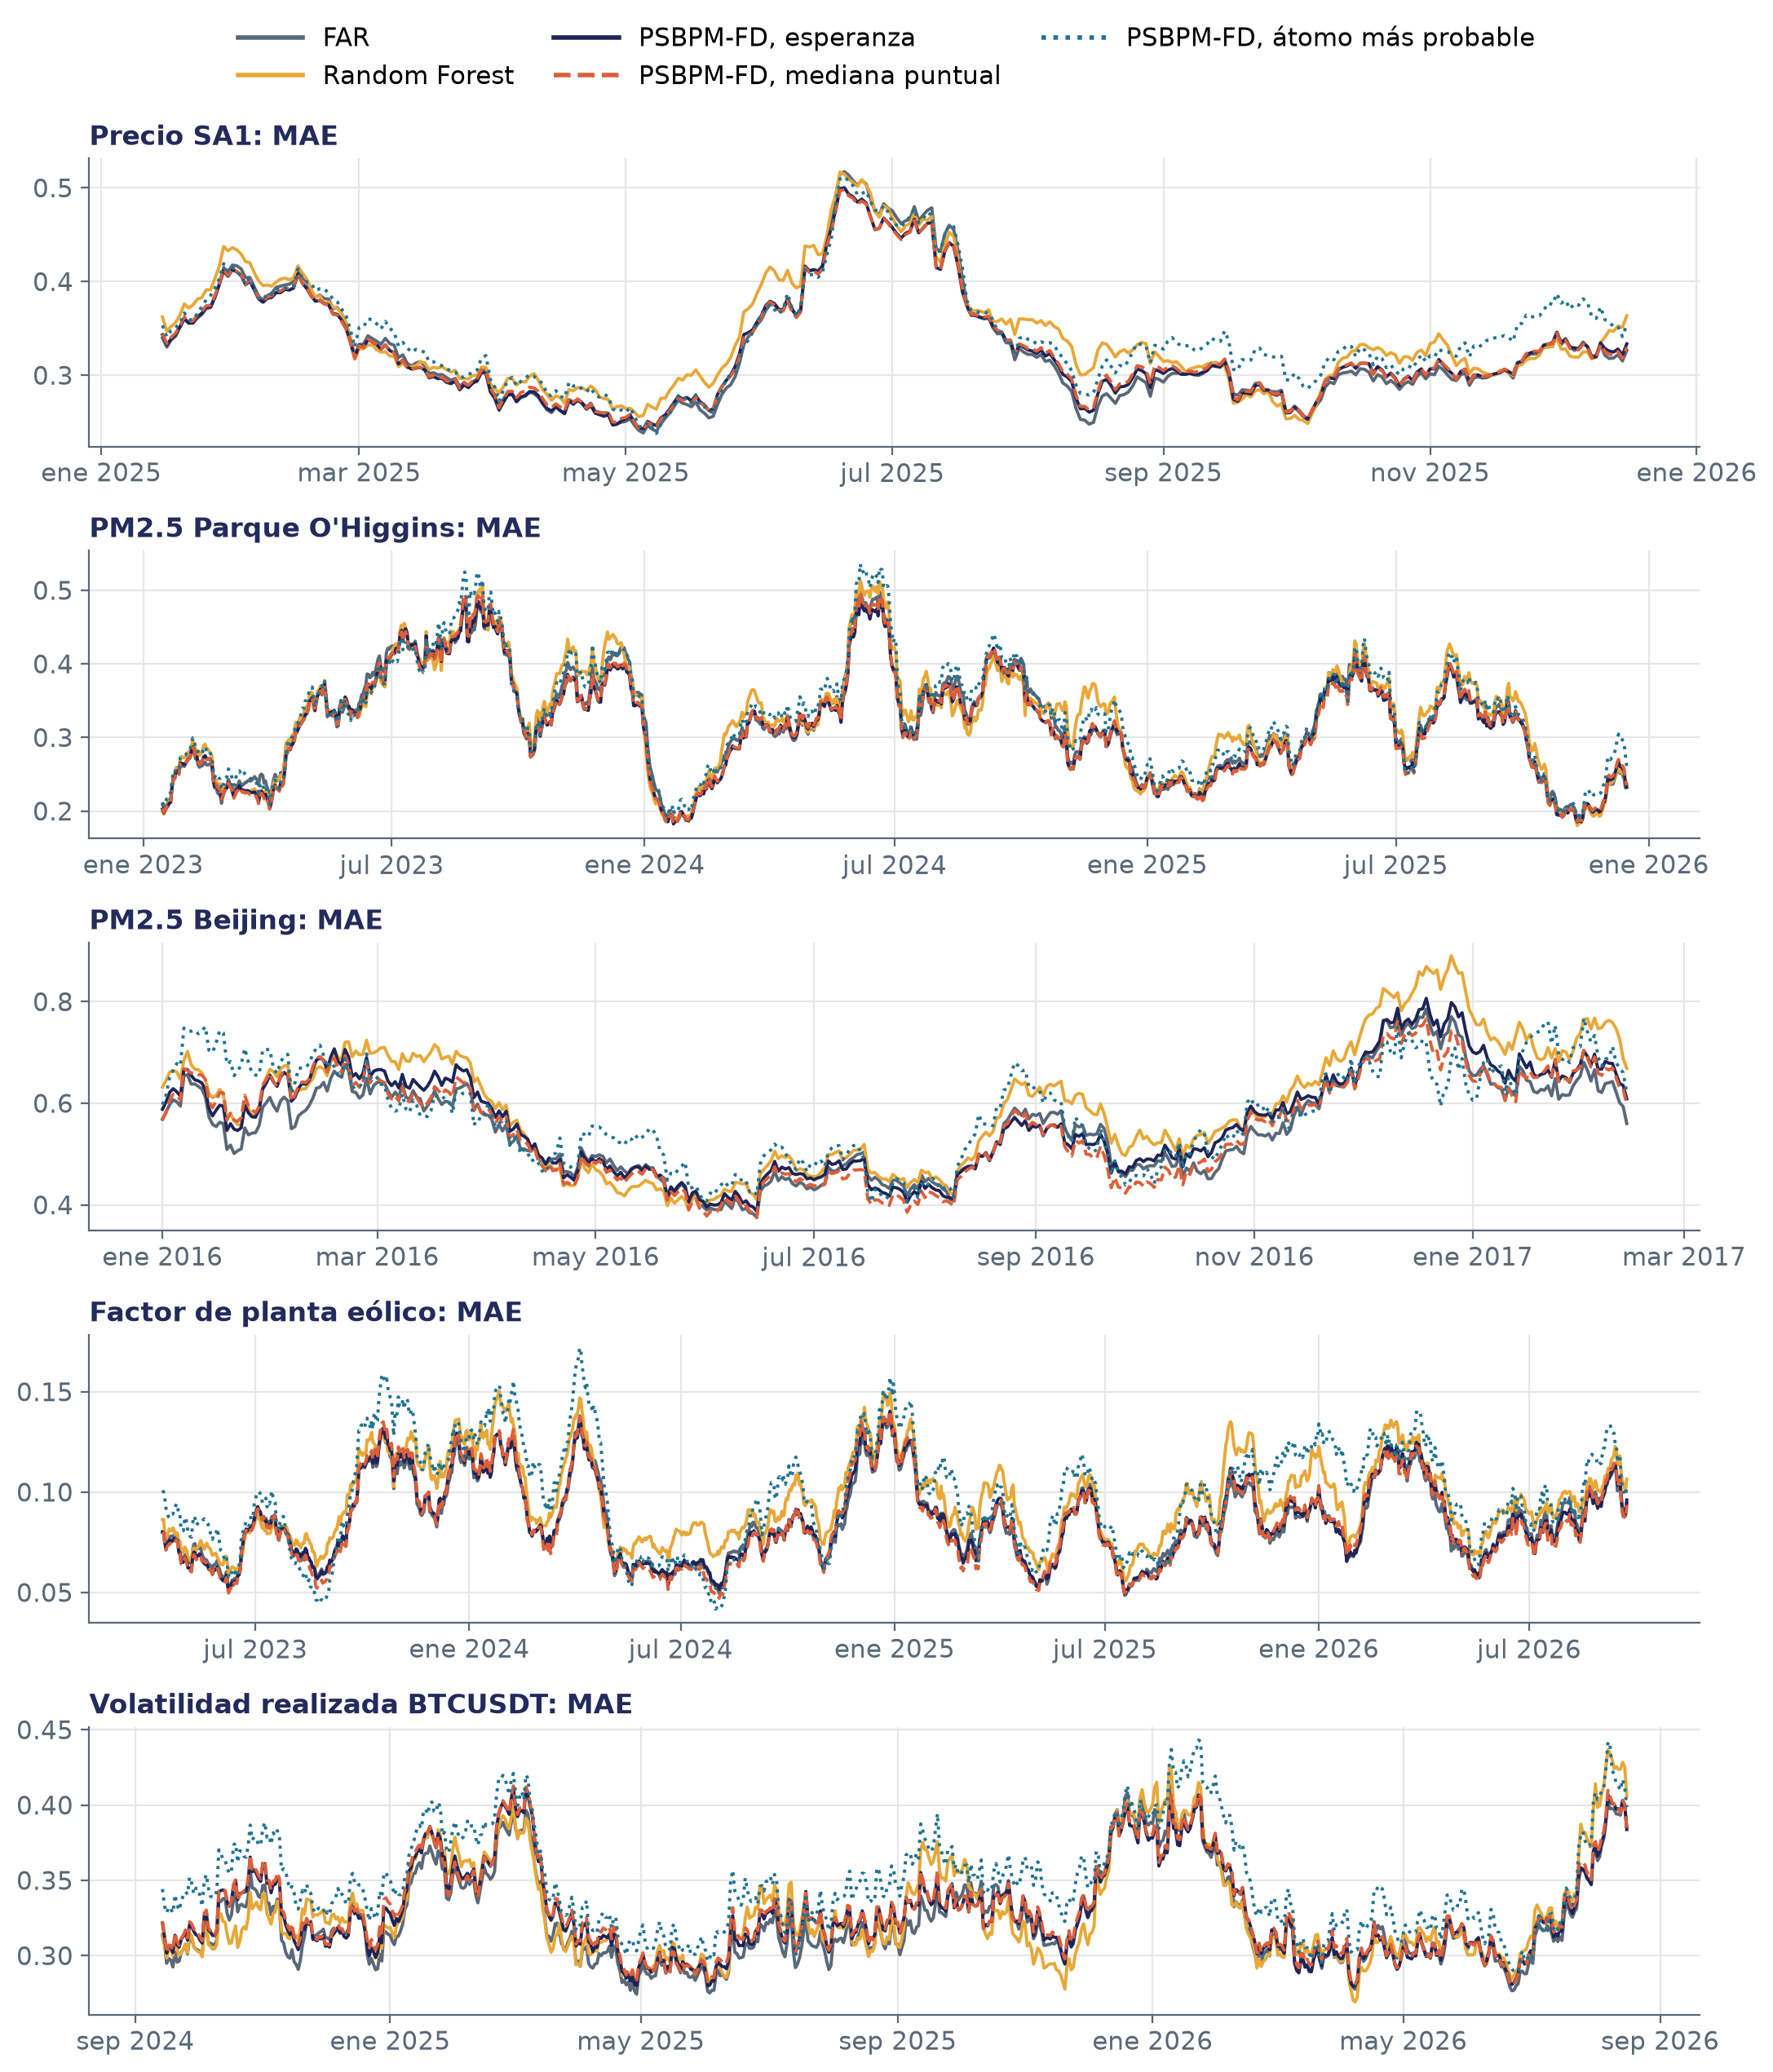
\includegraphics[width=\textwidth,height=0.85\textheight,keepaspectratio]{IMG/aneD_00/aneD_00_ventana_mae_w30.png}
\caption{MAE sobre la ventana móvil del bloque de prueba de los tres predictores del PSBPM-FD, el FAR y el Random Forest, por serie ($M = 10$, $w = 30$).}
\label{fig:aneD_ventana_mae}
\end{figure}

La Figura~\ref{fig:aneD_ventana_mae} muestra que las curvas de error de los cinco modelos se mueven juntas en todas las series: los períodos difíciles, como los meses de precios altos de junio y julio de 2025 en la SA1, los inviernos en las dos series de PM2.5 y en la eólica, lo son para todos los modelos, y las diferencias entre ellos son pequeñas frente a la variación del error a lo largo del bloque de prueba.

\section{Intervalos de predicción}
\label{aneD_00_03_intervalos}

Los Cuadros~\ref{tab:aneD_bloqueB_winkler} a~\ref{tab:aneD_bloqueB_ventanas} comparan las tres construcciones de intervalo del PSBPM-FD con la banda gaussiana del FAR, como en la Sección~\ref{04_03_02_intervalos}.

% Fuente: 99_resumen_bloqueB_min_max_prom.csv del barrido (test, M = 10).
\begin{table}[H]
\centering\small
\setlength{\tabcolsep}{3.5pt}
\caption{Winkler y MPIW en el bloque de prueba por serie y construcción ($M = 10$, $w = 30$). En negrita el menor Winkler de cada serie.}
\label{tab:aneD_bloqueB_winkler}
\begin{tabular}{l cccc cccc}
\hline
 & \multicolumn{4}{c}{Winkler} & \multicolumn{4}{c}{MPIW} \\
Serie & FAR & Equi. & HDR & Simult. & FAR & Equi. & HDR & Simult. \\
\hline
Precio SA1 & 2.374 & \textbf{2.354} & 2.361 & 2.977 & 1.872 & 1.881 & 1.885 & 2.870 \\
PM2.5 O'Higgins & 2.484 & \textbf{2.421} & 2.441 & 2.696 & 1.645 & 1.692 & 1.687 & 2.450 \\
PM2.5 Beijing & 3.883 & \textbf{3.522} & 3.717 & 4.169 & 2.710 & 2.852 & 2.847 & 3.986 \\
Eólica & \textbf{0.581} & 0.605 & 0.622 & 0.730 & 0.454 & 0.488 & 0.487 & 0.674 \\
Volatilidad BTC & \textbf{2.075} & 2.076 & 2.075 & 2.608 & 1.634 & 1.735 & 1.739 & 2.597 \\
\hline
\end{tabular}
\end{table}

\begin{table}[H]
\centering\small
\setlength{\tabcolsep}{3.5pt}
\caption{PICP y PICPB en el bloque de prueba por serie y construcción ($M = 10$, $w = 30$). Nivel nominal $0.95$.}
\label{tab:aneD_bloqueB_picp}
\begin{tabular}{l cccc cccc}
\hline
 & \multicolumn{4}{c}{PICP} & \multicolumn{4}{c}{PICPB} \\
Serie & FAR & Equi. & HDR & Simult. & FAR & Equi. & HDR & Simult. \\
\hline
Precio SA1 & 0.956 & 0.956 & 0.956 & 0.994 & 0.717 & 0.696 & 0.702 & 0.947 \\
PM2.5 O'Higgins & 0.937 & 0.942 & 0.941 & 0.981 & 0.676 & 0.686 & 0.696 & 0.901 \\
PM2.5 Beijing & 0.933 & 0.939 & 0.933 & 0.980 & 0.786 & 0.763 & 0.763 & 0.926 \\
Eólica & 0.946 & 0.955 & 0.956 & 0.985 & 0.783 & 0.808 & 0.825 & 0.940 \\
Volatilidad BTC & 0.944 & 0.954 & 0.955 & 0.995 & 0.633 & 0.673 & 0.677 & 0.951 \\
\hline
\end{tabular}
\end{table}

\begin{table}[H]
\centering\small
\setlength{\tabcolsep}{3pt}
\caption{Cambio relativo del Winkler y del MPIW respecto del FAR por serie y construcción. Negativo es mejor que el FAR.}
\label{tab:aneD_bloqueB_ganancia}
\begin{tabular}{l cc cc cc}
\hline
 & \multicolumn{2}{c}{Equi-colas} & \multicolumn{2}{c}{Máxima densidad} & \multicolumn{2}{c}{Simultánea} \\
Serie & Winkler & MPIW & Winkler & MPIW & Winkler & MPIW \\
\hline
Precio SA1 & $-0.8\%$ & $+0.5\%$ & $-0.5\%$ & $+0.7\%$ & $+25.4\%$ & $+53.3\%$ \\
PM2.5 O'Higgins & $-2.5\%$ & $+2.9\%$ & $-1.7\%$ & $+2.5\%$ & $+8.5\%$ & $+48.9\%$ \\
PM2.5 Beijing & $-9.3\%$ & $+5.3\%$ & $-4.3\%$ & $+5.1\%$ & $+7.4\%$ & $+47.1\%$ \\
Eólica & $+4.2\%$ & $+7.5\%$ & $+7.0\%$ & $+7.2\%$ & $+25.7\%$ & $+48.5\%$ \\
Volatilidad BTC & $+0.1\%$ & $+6.2\%$ & $0.0\%$ & $+6.4\%$ & $+25.7\%$ & $+59.0\%$ \\
\hline
\end{tabular}
\end{table}

% Fuente: 81_ventana_bloqueB_w30.csv (test, sin ventanas que cruzan T0).
\begin{table}[H]
\centering\small
\setlength{\tabcolsep}{3.5pt}
\caption{Fracción de ventanas de prueba en que cada banda tiene el menor Winkler, y en que cada banda del PSBPM-FD tiene un Winkler menor que el del FAR.}
\label{tab:aneD_bloqueB_ventanas}
\begin{tabular}{l cccc ccc}
\hline
 & \multicolumn{4}{c}{La mejor banda} & \multicolumn{3}{c}{Gana al FAR} \\
Serie & FAR & Equi. & HDR & Simult. & Equi. & HDR & Simult. \\
\hline
Precio SA1 & 39\% & 35\% & 19\% & 7\% & 60\% & 52\% & 8\% \\
PM2.5 O'Higgins & 32\% & 35\% & 16\% & 17\% & 61\% & 57\% & 24\% \\
PM2.5 Beijing & 20\% & 78\% & 3\% & 0\% & 80\% & 68\% & 28\% \\
Eólica & 64\% & 20\% & 16\% & 1\% & 34\% & 30\% & 1\% \\
Volatilidad BTC & 53\% & 25\% & 21\% & 0\% & 44\% & 42\% & 2\% \\
\hline
\end{tabular}
\end{table}

En los intervalos el resultado depende de la serie. La banda equi-colas del PSBPM-FD baja el Winkler del FAR en tres de las cinco series: con claridad en el PM2.5 de Beijing, un $9.3\%$ y en el $80\%$ de las ventanas, y por poco en el PM2.5 de Parque O'Higgins y en el precio SA1, un $2.5\%$ y un $0.8\%$, en alrededor del $60\%$ de las ventanas. En la volatilidad de BTC empatan, y en la eólica el FAR es mejor, un $4\%$ y en dos de cada tres ventanas. La banda del PSBPM-FD es algo más ancha que la del FAR en todas las series, entre un $0.5\%$ y un $7.5\%$ en MPIW, de modo que donde gana el Winkler lo hace porque la penalización por no cubrir la curva baja más de lo que sube el ancho. La banda de máxima densidad queda cerca de la equi-colas, porque con predictivas unimodales ambas construcciones se parecen, y se separa sobre todo en Beijing, la serie de predictiva asimétrica. La banda simultánea es la única que se acerca al nivel nominal en el PICPB, entre $0.90$ y $0.95$, frente a valores entre $0.63$ y $0.83$ de las bandas puntuales, y paga esa cobertura con un ancho cerca de un $50\%$ mayor y el peor Winkler en todas las series.

% Fuente: 81_ventana_bloqueB_w30.csv de cada serie (test).
\begin{figure}[H]
\centering
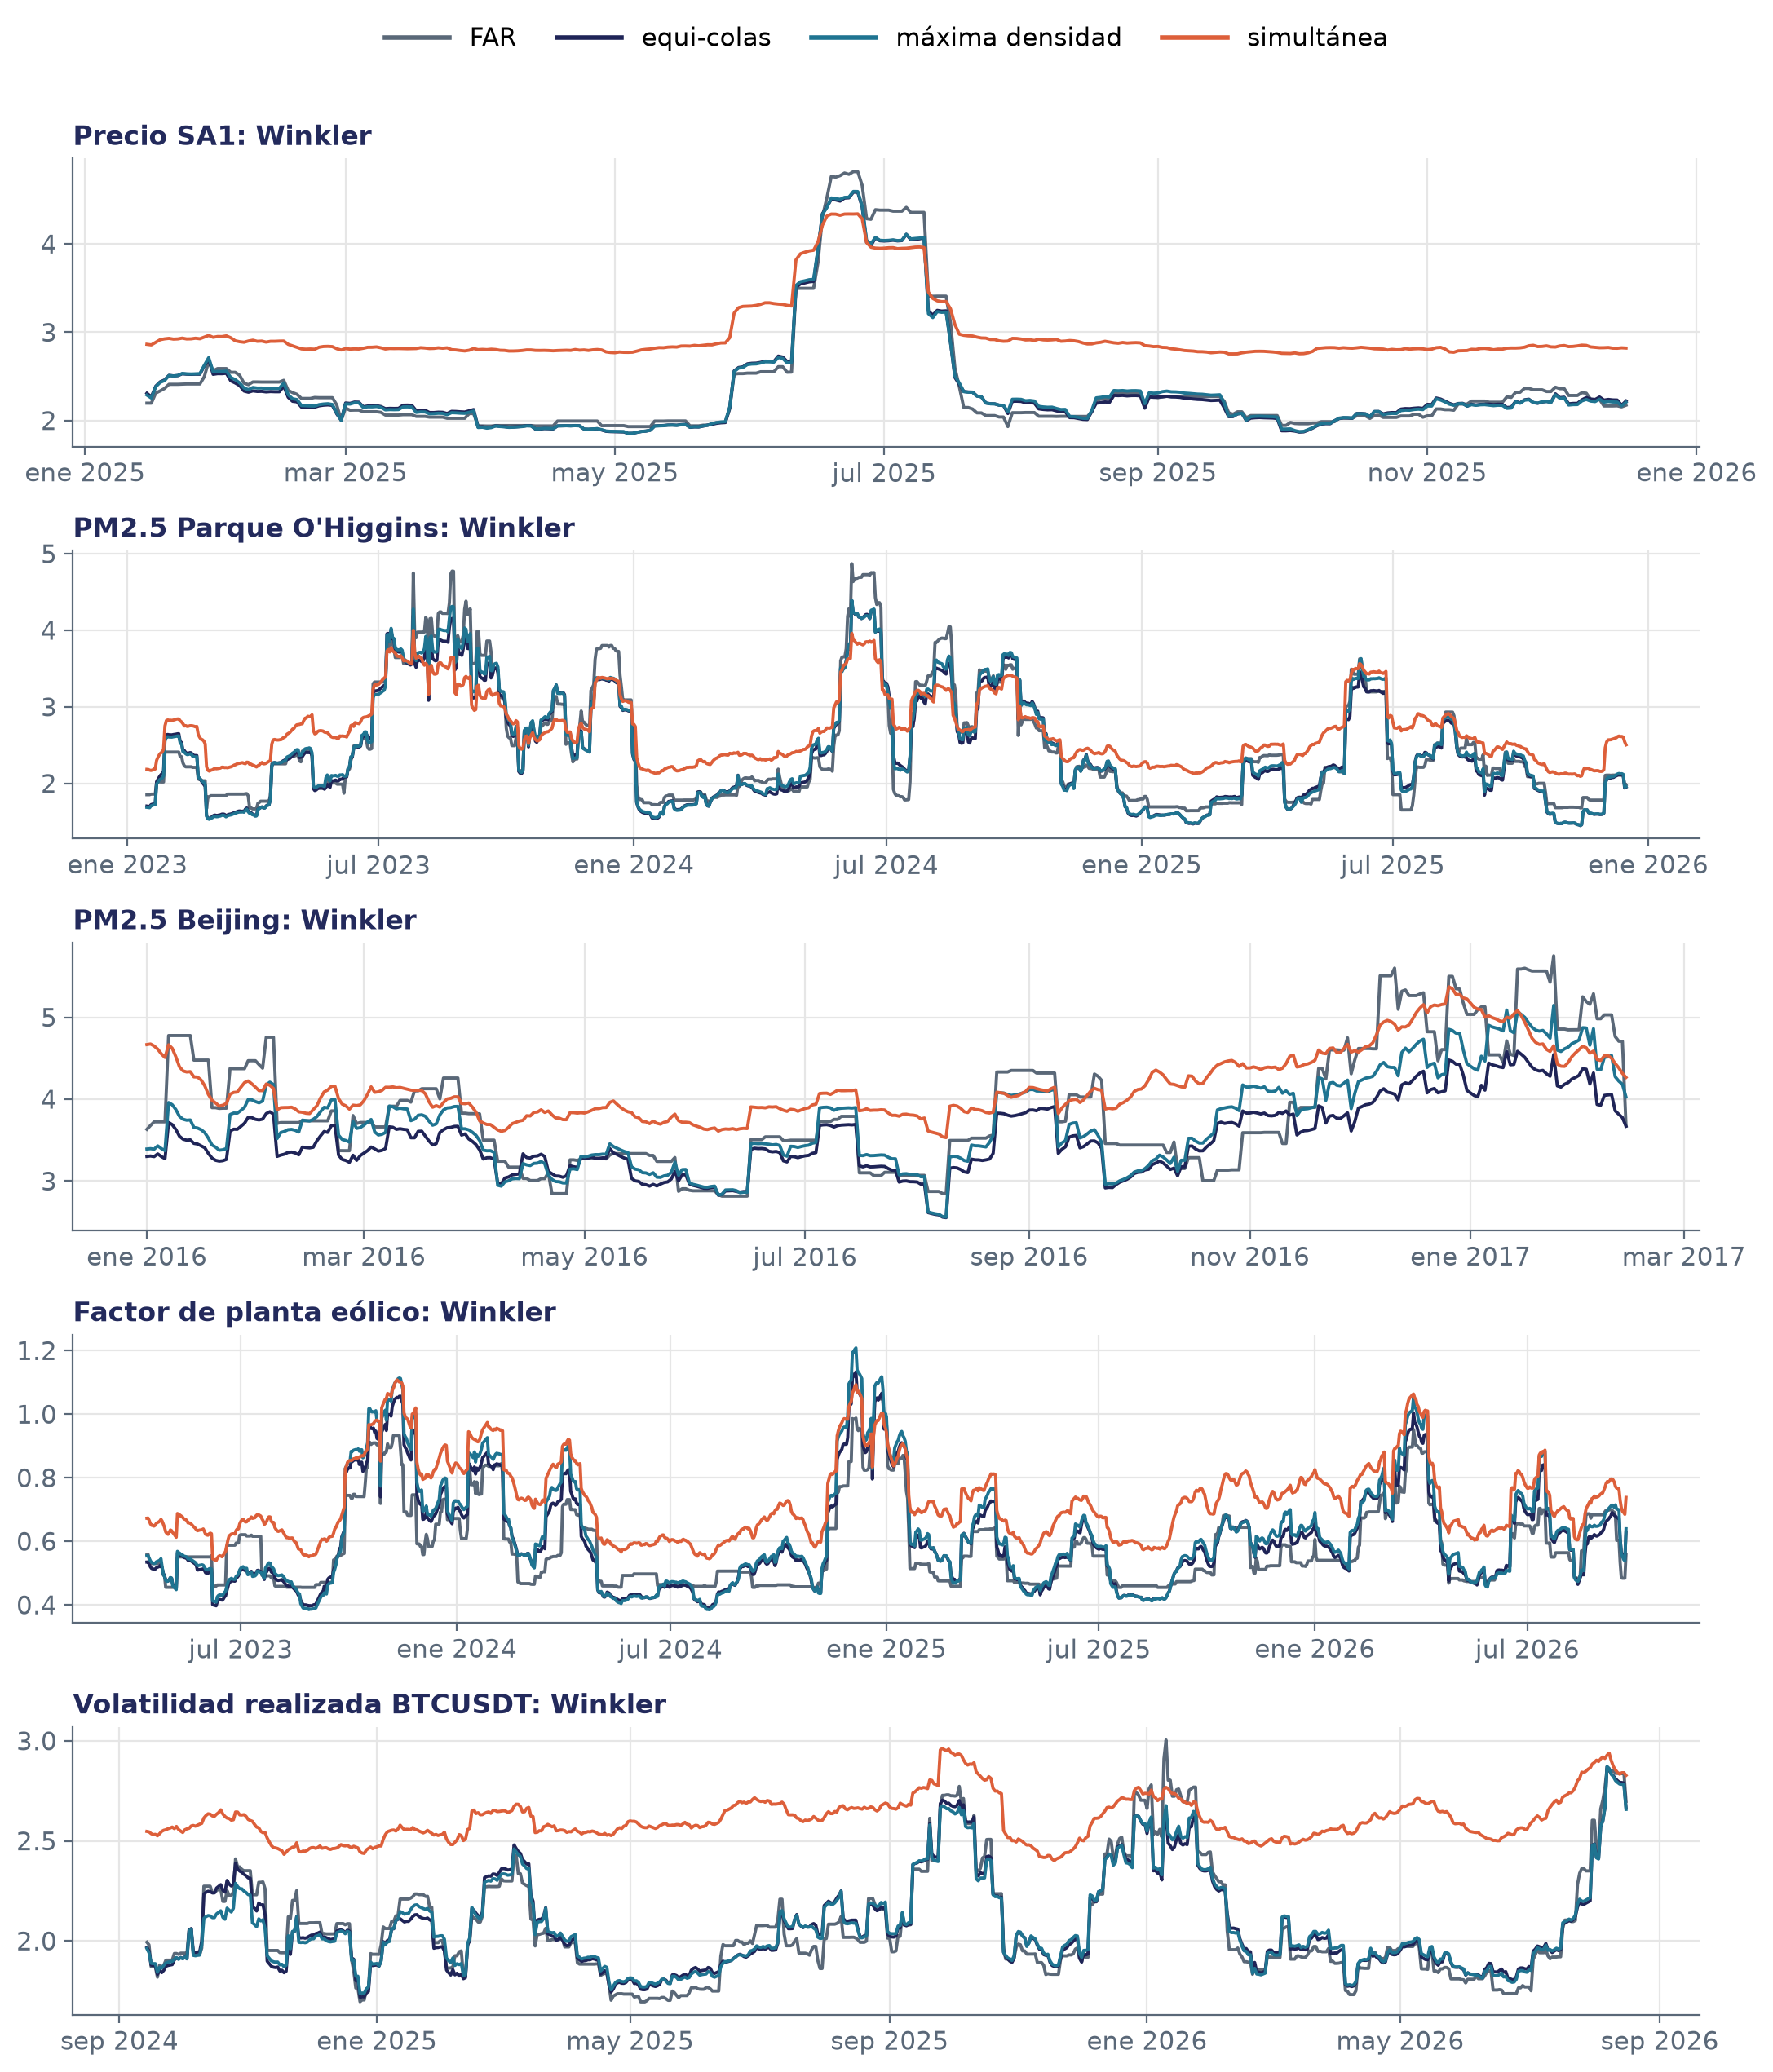
\includegraphics[width=\textwidth,height=0.85\textheight,keepaspectratio]{IMG/aneD_00/aneD_00_ventana_winkler_w30.png}
\caption{Winkler sobre la ventana móvil del bloque de prueba de las tres construcciones del PSBPM-FD y de la banda del FAR, por serie ($M = 10$, $w = 30$).}
\label{fig:aneD_ventana_winkler}
\end{figure}

La Figura~\ref{fig:aneD_ventana_winkler} muestra dónde se produce la diferencia. En el PM2.5 de Beijing la banda equi-colas queda bajo la del FAR en la mayor parte del bloque de prueba, con la mayor distancia en los dos inviernos. En el precio SA1 y en el PM2.5 de Parque O'Higgins las bandas del PSBPM-FD quedan bajo la del FAR en los tramos de mayor Winkler, los meses de precios altos de 2025 en la SA1 y los inviernos en Santiago, y se confunden con ella en el resto. En la eólica, en cambio, la banda del FAR es la mejor en dos de cada tres ventanas, repartidas a lo largo del bloque, y en la volatilidad de BTC las bandas puntuales no se distinguen.

\section{Comportamientos predictivos}
\label{aneD_00_04_comportamientos}

El Cuadro~\ref{tab:aneD_K} resume cuántos comportamientos declara el modelo en el bloque de prueba de cada serie.

% Fuente: 102_K_por_M.csv del barrido (test, M = 10); fechas de los orígenes con K = 2 en 65_comportamientos_calendario.csv.
\begin{table}[H]
\centering\small
\setlength{\tabcolsep}{3.5pt}
\caption{Distribución de $K_t$ en el bloque de prueba por serie ($M = 10$) y número de orígenes con más de un comportamiento.}
\label{tab:aneD_K}
\begin{tabular}{l c ccc c}
\hline
Serie & Orígenes & $K_t = 1$ & $K_t = 2$ & $K_t \ge 3$ & Orígenes con $K_t \ge 2$ \\
\hline
Precio SA1 & 365 & 99.7\% & 0.3\% & 0.0\% & 1 \\
PM2.5 O'Higgins & 1096 & 99.5\% & 0.5\% & 0.0\% & 5 \\
PM2.5 Beijing & 439 & 100.0\% & 0.0\% & 0.0\% & 0 \\
Eólica & 1290 & 99.9\% & 0.1\% & 0.0\% & 1 \\
Volatilidad BTC & 731 & 100.0\% & 0.0\% & 0.0\% & 0 \\
\hline
\end{tabular}
\end{table}

En las cinco series la predictiva tiene un solo comportamiento en al menos el $99.5\%$ de los orígenes de prueba, y en Beijing y en la volatilidad de BTC en todos. Los pocos orígenes con dos comportamientos coinciden con días extremos: el único de la SA1 es el 3 de julio de 2025, con un precio máximo de casi 3900 AUD/MWh; el de la eólica es un día de temporal, y tres de los cinco del PM2.5 de Parque O'Higgins son días sobre la norma diaria, todos entre mayo y julio. Con un solo comportamiento el pronóstico por comportamiento coincide con la esperanza, y por eso no se reporta. El resultado es el que se esperaba: sin un estado oculto que separe perfiles de la curva siguiente, la mezcla no produce comportamientos, y la ventaja del PSBPM-FD se reduce a la que su banda obtiene de adaptar el ancho al estado del proceso, clara en Beijing, pequeña en el PM2.5 de Santiago y en la SA1, y nula o en contra en la volatilidad de BTC y en la eólica, más una mejora pequeña del error puntual en el PM2.5 de Santiago.
